\section{Results: Stage V1}
\label{sec:results}
All numbers come from the reproduction script on the original result files. Study~A has \nPos{} paired positions, Study~B 500 games and Study~C 1{,}000 puzzles.

\subsection{Search versus System~1 alone (descriptive)}
\label{sec:search-value}
Always searching lowers ACPL from \acplLaya{} to \acplSTwo{}: a paired difference of \dAcpl{}\cp\ (95\% CI [\dAcplLo, \dAcplHi]; [\dClLo, \dClHi] resampling games) at \costRatio$\times$ the cost (\msLaya\ to \msSTwo\,ms; Table~\ref{tab:agents}). The standardised effect is small ($d_z=\cohenDz$). Blunders fall from \blunLaya\% to \blunSTwo\%. \ag{mcts_uniform}, the value network without System~1, is far worse (ACPL \acplMcts{}), so search is useful only because it inherits System~1's scores. The average is carried by a minority of positions: search changes System~1's move in \fracChanged\% (\nChanged{}); of these \nBetter{} are better, \nWorse{} worse and \nEqual{} equal. Capping CPL at 200\cp\ shrinks the difference to \capTwoHundred\cp, and search repairs \nFixed{} of \nLayaBlunder{} System~1 blunders (\fixedPct\%) while introducing \nIntro{} new ones.

\begin{table}[t]
\centering
\caption{Study~A (test split, $n=\nPos$ positions per agent). System~1 = \ag{laya_only}, Always~S2 = \ag{always_s2}, MCTS only = \ag{mcts_uniform}; time is mean wall time per move.}
\label{tab:agents}
\small
\footnotesize\setlength{\tabcolsep}{4pt}\begin{tabular}{lrrr}
\toprule
 & System 1 & Always S2 & MCTS only \\
\midrule
ACPL (cp) & 107.9 & 103.1 & 235.4 \\
\quad 95\% CI & [101.0, 114.4] & [96.6, 109.6] & [226.0, 245.0] \\
Median CPL (cp) & 28 & 26 & 121 \\
Good moves (\%) & 48.6 & 49.7 & 31.2 \\
Blunders (\%) & 17.3 & 16.6 & 42.4 \\
Top-1 agreement (\%) & 26.2 & 27.0 & 17.7 \\
Mean ms per move & 468 & 1499 & 1042 \\
\bottomrule
\end{tabular}

\end{table}

\subsection{Is confidence informative? (\Hone{}, \Hfour{})}
The AUROC of confidence for predicting a good move is \aucConf{} [\aucConfLo, \aucConfHi], close to its validation value (\valAuc{}); it exceeds the legal-move baseline (\aucBase{}) only by \aucDiff{} [\aucDiffLo, \aucDiffHi], an interval including zero, so \Hone{} is met only in its first clause. The good-move rate rises with confidence from about 42\% to 91\%. \Hfour{} fails in the opposite direction: the blunder rate is \qOne\% in the lowest-confidence quartile and \qFour\% in the highest (ratio \qRatio{} [\qRatioLo, \qRatioHi]). One post hoc reading is that low-confidence positions have many near-equal moves, so errors there are cheap, whereas large errors concentrate in sharp positions: \ag{laya_only} has ACPL \acplSharp\cp\ where the Stockfish gap exceeds 300\cp, and its mean confidence there is \confSharp{} against \meanConfAll{} overall.

\subsection{Does confidence gating beat random gating? (\Htwo{}, \Hthree{})}
\label{sec:h2}
\begin{figure*}[t]
\centering
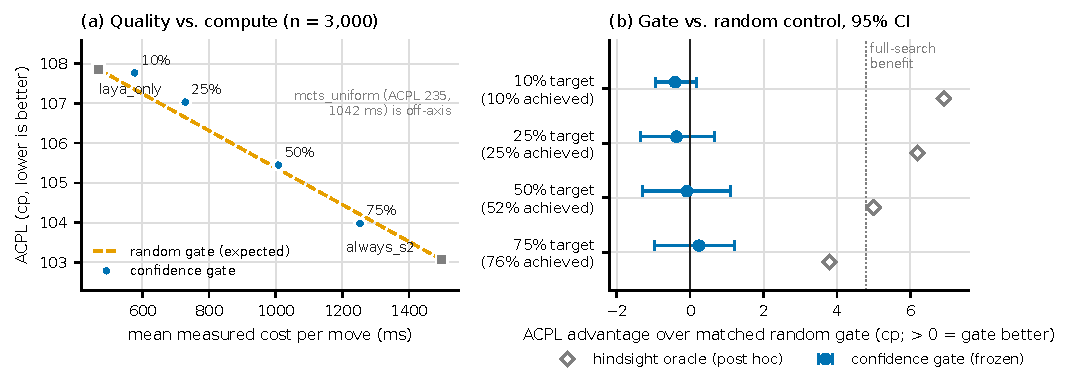
\includegraphics[width=\textwidth]{fig_tradeoff}
\caption{Quality--compute trade-off, Study~A. (a) ACPL against measured cost for the frozen confidence gate at its four achieved rates; the dashed line is the expected value of a random gate. (b) ACPL advantage of the confidence gate over a random gate at the same rate (analytic expectation; 95\% bootstrap interval). Hollow diamonds are a post hoc hindsight oracle and are not achievable.}
\label{fig:tradeoff}
\end{figure*}
\begin{table*}[t]
\centering
\caption{\Htwo{} and \Hthree{} at the frozen thresholds (Study~A). $^{\dagger}$Expectation over random gates at the achieved rate. Advantage $>0$ favours the confidence gate. Recovery $R=(\mathrm{ACPL}_{S1}-\mathrm{ACPL}_{gate})/(\mathrm{ACPL}_{S1}-\mathrm{ACPL}_{S2})$; a random gate has expected $R$ equal to its search rate.}
\label{tab:h2}
\small
\begin{tabular}{rrrrcccr}
\toprule
Target & Achieved & ACPL & ACPL & Gate $-$ random advantage & Holm & Recovery $R$ & Search time \\
rate (\%) & rate (\%) & gate & random$^{\dagger}$ & (cp, 95\% CI) & $p$ & [95\% CI] & used (\%) \\
\midrule
10 & 10.5 & 107.77 & 107.35 & \ensuremath{-}0.41 [\ensuremath{-}0.96, 0.17] & -- & 0.02 [\ensuremath{-}0.13, 0.15] & 10.5 \\
25 & 25.0 & 107.03 & 106.66 & \ensuremath{-}0.37 [\ensuremath{-}1.37, 0.67] & 1.00 & 0.17 [\ensuremath{-}0.06, 0.40] & 25.2 \\
50 & 52.1 & 105.45 & 105.36 & \ensuremath{-}0.09 [\ensuremath{-}1.30, 1.11] & 1.00 & 0.50 [0.24, 0.79] & 52.3 \\
75 & 75.9 & 103.98 & 104.22 & 0.24 [\ensuremath{-}0.96, 1.22] & -- & 0.81 [0.56, 1.04] & 76.2 \\
\bottomrule
\end{tabular}

\end{table*}
At no rate does the gate beat its matched random control (Fig.~\ref{fig:tradeoff}, Table~\ref{tab:h2}). At the two pre-registered rates the advantage is \advTf{}\cp\ [\advTfLo, \advTfHi] at \rateTf\% and \advFifty{}\cp\ [\advFiftyLo, \advFiftyHi] at \rateFifty\%; both Holm-adjusted $p$-values are 1.0, so \Htwo{} is not supported. The 10\% and 75\% rates agree (\advTen{}, \advSf{}\cp). The absence of an advantage is not equivalence: the minimum detectable advantage is \mdeTen--\mdeFifty\cp, and the data are compatible with an advantage of up to \maxAdvHi\cp\ (\maxAdvHiPct\% of the full benefit). \Hthree{} is not supported: at \rateFifty\% search the gate recovers $R=\RFifty$ [\RFiftyLo, \RFiftyHi] of the benefit, but uses \shareFifty\% of the search time and a random gate is expected to recover $R=\randRFifty$. Recovery is proportional to the search budget.

\subsection{Playing strength (\Hsix{}) and puzzles (\Hfive{})}
\label{sec:studyb}
\begin{table}[t]
\centering
\caption{Study~B ratings on the anchor's nominal scale, pooled over all 500 games (anchor 1320 fixed). Each agent played 200 games; the last column is its score in the 50 games against the anchor (Wilson interval).}
\label{tab:elo}
\small
\footnotesize\setlength{\tabcolsep}{3pt}\begin{tabular}{lrrr}
\toprule
Agent & Elo$^{\ddagger}$ [95\% CI] & Score (\%) & vs.\ anchor (\%) \\
\midrule
\texttt{laya\_only} & 904 [832, 958] & 46.8 & 11 (5--23) \\
\texttt{always\_s2} & 887 [821, 938] & 44.2 & 6 (2--16) \\
\texttt{hybrid\_s2\_50} & 879 [809, 932] & 43.0 & 8 (3--19) \\
\texttt{mcts\_uniform} & 734 [668, 783] & 22.5 & 1 (0--9) \\
\bottomrule
\end{tabular}

\end{table}
Ratings (Table~\ref{tab:elo}) are \ag{laya_only} \eloLaya{} [\eloLayaLo, \eloLayaHi], \ag{always_s2} \eloAlw{}, \ag{hybrid_s2_50} \eloHyb{}, \ag{mcts_uniform} \eloMu{}. The paired contrast for \Hsix{} is \eDHL{} Elo [\eDHLLo, \eDHLHi] for hybrid minus \ag{laya_only}: the estimate favours System~1 alone, from three decisive head-to-head losses of the hybrid and none won (\hhWins{} wins, \hhDraws{} draws, \hhLosses{} losses), so we read it as weak evidence against \Hsix{}, not as evidence that the hybrid is weaker. Three qualifications apply. Every agent scored only \ancMu--\ancLaya\% against the single anchor, so absolute ratings are extrapolations. \rrThree{} of \rrN{} round-robin games (\rrThreePct\%) ended in threefold repetition and only \nUniqSeq{} distinct move sequences occur among 500 games, so the effective number of games is well below 500. And in games \ag{hybrid_s2_50} used System~2 on \hybSysShare\% of moves, far above its \rateFifty\% rate in Study~A, because game positions have low confidence.

On puzzles, search adds little: pooled solve rates are \puzPoolLaya\% for \ag{laya_only}, \puzPoolHyb\% for \ag{hybrid_s2_50} and \puzPoolAlw\% for \ag{always_s2} (paired difference \puzDAlw{} points [\puzDAlwLo, \puzDAlwHi], McNemar $p=\puzPAlw$), and no bucket differs by more than \puzMaxBucket{} points. This bounds the effect to one or two points; it does not show search is useless on tactics. \Hfive{} fails in the opposite direction: the 50\% gate sends \trigPuz\% of puzzles to search against \trigGames\% of game positions, plausibly because forcing positions have a standout top move and hence high confidence.

\subsection{Exploratory: why confidence fails to locate search gains}
\label{sec:explore}
Everything here was computed after the test outcomes were visible and changes no verdict. Low confidence flags where search \emph{changes} the move (AUROC \aucChange; override rate \decChangeLow\% in the least confident decile against \decChangeHigh\% in the most), but among changed positions it does not predict improvement (AUROC \aucImprove, Spearman $\rho=\rhoChanged$), and the average gain of an override is larger where System~1 is confident (\chGainHigh\cp\ against \chGainLow\cp). Overall, confidence and search gain have $\rho=\rhoGain$ [\rhoGainLo, \rhoGainHi], with \fracGainZero\% of gains exactly zero. Gains concentrate in endgames (\gainEnd\cp, Holm $p=\pHolmEnd$) and in positions where one move is more than 300\cp\ better than the next (\gainSharp\cp, $n=\nSharp$, Holm $p=\pHolmSharp$); positions with gap above 300\cp\ (\fracSharp\%) supply \shareSharp\% of total gain. These are the positions where System~1 is \emph{more} confident, so confidence behaves as a forcedness signal and a gate that triggers on low confidence points away from where search helps. Gates on inverted confidence, legal-move count or even the Stockfish gap stay within about 1\cp\ of random. A hindsight oracle reaches ACPL \oracleAcpl{} at a 10\% rate (\oracleCostPct\% of the cost of always searching), below always searching (\acplSTwo{}), but it is selected and scored on the same noisy judgments, so it is a ceiling and not an achievable gate.
